% Copyright (c) 2019 Guoli Ding
%
% Distributed under the Boost Software License, Version 1.0. (See accompanying
% file LICENSE_1_0.txt or copy at http://www.boost.org/LICENSE_1_0.txt)
%

\documentclass[10pt]{article}
\renewcommand{\baselinestretch}{1.1}
\usepackage{fullpage,amssymb,amsmath,graphicx,color}

\parskip 8pt

\begin{document}

\centerline{\LARGE DAG scheduling} 

\bigskip
\centerline{\large Guoli Ding and Rod Tohid}

\medskip
\centerline{\large \today}

\bigskip
\noindent{\bf The inputs.} \\ 
\indent $\bullet$ \ A positive integer $m$, indicating that there are $m$
machines available. \\  
\indent $\bullet$ \ An acyclic directed graph $D=(V,E)$, known as a DAG. Here a
vertex represents a job and a directed \makebox[24pt]{} edge $e=uv$ indicates
that job $v$ cannot start before job $u$ finishes.\\ 
\indent $\bullet$ \ A nonnegative weight function $\ell$ on $V\cup E$, where
$\ell_v$ indicates the amount of time required to finish \makebox[23pt]{} job
$v$, and $\ell_{uv}$ indicates the amount of time required for $v$ to access $u$
if $u,v$ are located on different \makebox[23pt]{} machines. 

\noindent {\bf Assumptions.} \\ 
\indent $\bullet$ \ A machine can process at most one job at a time. \\ 
\indent $\bullet$ \ If a machine starts a job then it has to finish the job
before it can start another job. In particular, \makebox[23pt]{} this implies
that a job can only be completed by one machine.\\ 
\indent $\bullet$ \ For each job $v$, the weight $\ell_v$ is the same on every
machine. That is, a job can be done by any machine \makebox[23pt]{} with the
same amount of time, or simply put, the machines are identical.  \\ 
\indent $\bullet$ \ For any edge $e=uv$, the weight $\ell_e$ remains the same no
matter which two machines process $u$ and $v$. \makebox[23pt]{} In other words,
the communication channels are identical.

\noindent{\bf The problem.} \\ 
\indent $\bullet$ \ Decide which job goes to which machine. \\ 
\indent $\bullet$ \ Decide a starting time for each job.\\ 
\indent $\bullet$ \ Minimize the final completion time of all jobs.

\noindent{\bf Linear programming formulation.} Let $M_1,...,M_m$ denote the
machines and let $v_1,...,v_n$ denote the jobs. We introduce the following
variables. \\ 
\indent $\bullet$ \ $t_i$: the starting time for $v_i$\\ 
\indent $\bullet$ \ $T$: final finishing time\\  
\indent $\bullet$ \ $x_{ij}$: the assignment indicator, which is 1 if job $v_i$
is assigned to machine $M_j$, and is 0 if otherwise\\ 
\indent $\bullet$ \ $y_{ij}$: the time line indicator, which is 1 if $t_i\le
t_j$ and is 0 if $t_i>t_j$\\ 
\indent $\bullet$ \ $L$ : defined as the sum of $\ell$ over $V\cup E$, which is
the total amount of involved time \\ 
The following is the formulation.

$\min \ T$

\vspace{-5pt}
subject to:

\vspace{-6pt}
\makebox[15pt]{} $x_{i1}+x_{i2}+ \cdots + x_{im}=1$, \ \ $\forall v_i\in V$
\hfill (1)

\vspace{-4pt}
\makebox[15pt]{} $t_j-t_i-\ell_i\ge \ell_{ij}\max\{x_{ik}-x_{jk}:k=1,...,m\}$, \
\ $\forall v_iv_j\in E$ \hfill (2)

\vspace{-4pt}
\makebox[15pt]{} $t_j-t_i-\ell_i\ge
L(\max\{x_{ik}+x_{jk}-2:k=1,...,m\}+y_{ij}-1)$, \ \ $\forall v_i,v_j\in V$ with
$i<j$ \hfill (3a)

\vspace{-4pt}
\makebox[15pt]{} $t_i-t_j-\ell_j\ge
L(\max\{x_{ik}+x_{jk}-2:k=1,...,m\}-y_{ij})$, \ \ $\forall v_i,v_j\in V$ with
$i<j$ \hfill (3b)

\vspace{-4pt}
\makebox[15pt]{} $T\ge \max\{t_i+\ell_i: i=1,...,n\}$ \hfill (4)

\vspace{-4pt}
\makebox[15pt]{} $t_i\ge0$; \ $x_{ij}\in\{0,1\}$; $y_{ij}\in\{0,1\}$

\noindent Note that the number of variables is $n+1+mn+(^n_2)$ and the umber of
inequalities is $m(n^2+|E|-n)+3n$. Some of the inequalities/variables are
redundant and thus can be removed.

\noindent{\bf Greedy Algorithm.} \\ 
\indent $\bullet$ \ Keep tract of the set $R$ of ready jobs (with cleared
dependencies) \\ 
\indent $\bullet$ \ As soon as a machine becomes available, \\ 
\makebox[9mm]{} $\circ$ \ update $R$\\ 
\makebox[9mm]{} $\circ$ \ assign a job from $R$ to this machine\\ 
\indent $\bullet$ \ Repeat until all jobs are scheduled. 

\noindent{\sc Remarks.} \\ 
\indent $\bullet$ \ \parbox[t]{155mm}{At any point in time, let $F$ denote the
set of jobs that are finished (so $F=\emptyset$ in the very beginning). Then $R$
consists of jobs $v$ such that no edge of $D\backslash F$ is directed to $v$.
That is, the in-degree of $v$ is zero in $D\backslash F$.}\smallskip\\ 
\indent $\bullet$ \ \parbox[t]{155mm}{When assigning $v\in R$ 
to an available machine, there are many choices. We could develop different principles for making such a choice and let experiments decide which is better --this is further research. }


\medskip
\noindent{\bf An application.} Suppose we have a user program $\mathbb P$, by
which we mean a sequence of matrix operations (an example of $\mathbb P$ is
illustrated below). Program $\mathbb P$ can be expressed by a computation graph
$\mathbb G$ (which is essentially the execution tree) and this graph is a DAG
(as illustrated below). If we want to process $\mathbb P$ in $m$ machine then we
have exactly the DAG scheduling problem.


 
\vspace{15mm}\makebox[11mm]{} \fbox{\parbox[b]{29mm}{
Input: $A,B,C,D$;\medskip\\ 
\makebox[5pt]{} $E\ =\ A+B$;\\ 
\makebox[5pt]{} $F\ =\ C * E$; \\ 
\makebox[5pt]{} $G\ =\ E * D$; \\ 
\makebox[5pt]{} $F\ =\ F+G$;\medskip\\ 
Output: $F$}}

\vspace{-49mm}\makebox[55mm]{} 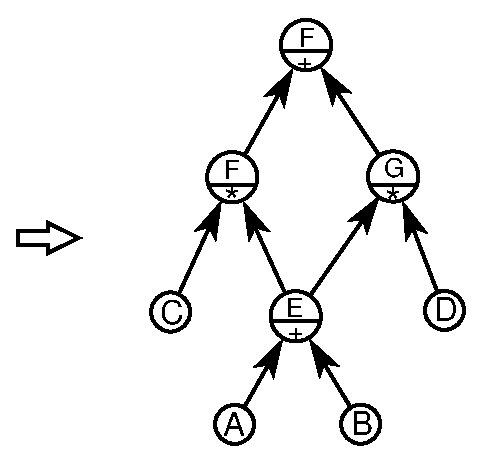
\includegraphics[scale=0.9]{executiong.eps}

\end{document}
